\documentclass{standalone}
\usepackage{tikz-network}
\begin{document}
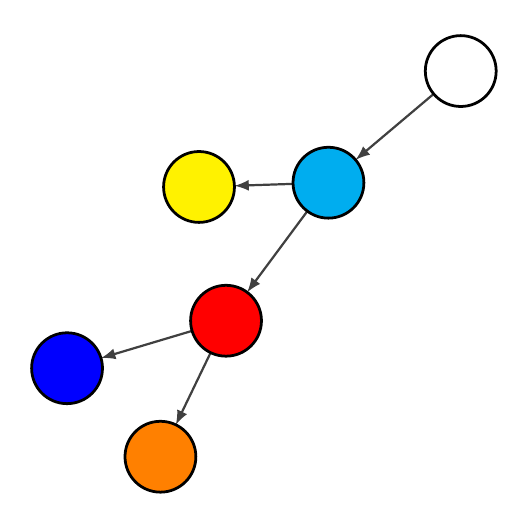
\begin{tikzpicture}
\clip (0,0) rectangle (6,6);
\Vertex[x=5.500,y=5.449,size=0.9,color=white,fontscale=0.857,shape=circle]{1}
\Vertex[x=3.820,y=4.031,size=0.9,color=cyan,fontscale=0.857,shape=circle]{2}
\Vertex[x=2.176,y=3.977,size=0.9,color=yellow,fontscale=0.857,shape=circle]{3}
\Vertex[x=2.519,y=2.278,size=0.9,color=red,fontscale=0.857,shape=circle]{4}
\Vertex[x=1.686,y=0.551,size=0.9,color=orange,fontscale=0.857,shape=circle]{5}
\Vertex[x=0.500,y=1.675,size=0.9,color=blue,fontscale=0.857,shape=circle]{6}
\Edge[,lw=0.8,bend=0,Direct](1)(2)
\Edge[,lw=0.8,bend=0,Direct](2)(3)
\Edge[,lw=0.8,bend=0,Direct](2)(4)
\Edge[,lw=0.8,bend=0,Direct](4)(5)
\Edge[,lw=0.8,bend=0,Direct](4)(6)
\end{tikzpicture}
\end{document}